%!TEX program = xelatex
\documentclass[12pt,a4paper]{article}
\usepackage{polyglossia}
\setmainlanguage[variant=mono]{greek}
\setotherlanguage{english}
\setmainfont[Mapping=tex-text]{GFS Elpis}
\usepackage{amsmath}
\usepackage{amsfonts}
\usepackage{amssymb}
\usepackage{amsthm}
\usepackage{listings}
\usepackage{float}
\usepackage{graphicx}
\usepackage{epstopdf}
\author{Γραμμένος Θεόδωρος}
\title{2η υποχρεωτική εργασία στο μάθημα της Αριθμητικής Ανάλυσης}
\date{ΑΕΜ: 3294}
\begin{document}
\maketitle
\subsection*{Άσκηση 5}
Για να προσεγγίσω θα πάρω τις παρακάτω τιμές του ημιτόνου με ακρίβεια 4 δεκαδικών ψηφίων
\begin{enumerate}
    \item $sin(0) = 0$
    \item $sin(\frac{23\pi}{60}) = 0.9336$
    \item $sin(\frac{\pi}{2}) = 1$
    \item $sin(\frac{71\pi}{90}) = 0.6157$
    \item $sin(\pi) = 0$
    \item $sin(\frac{13\pi}{12}) = -0.2588$
    \item $sin(\frac{239\pi}{180}) = -0.8572$
    \item $sin(\frac{3\pi}{2}) = -1$
    \item $sin(\frac{109\pi}{60}) = -0.5446$
    \item $sin(2\pi) = 0$
\end{enumerate}
Αρχικά, δημιοργούμε ένα script στο MATLAB το οποίο υπολογίζει μια εκτίμηση του ημιτόνου μιας γωνίας x χρησιμοποιώντας 
ένα πολυώνυμο Lagrange από τα παραπάνω 10 σημεία. Το αρχείο βρίσκεται στο scripts/ex1/lagrangeSin.m. Επίσης, στο αρχείο 
scripts/ex1/splineSin.m βρίσκεται η υλοποίηση με splines και στο scripts/ex1/leastSquareSin.m η υλοποίηση με τη μέθοδο ελαχίστων 
τετραγώνων. Στην μέθοδο ελαχίστων τετραγώνων χρησιμοποιείται πολυώνυμο 8ου βαθμού. Ο βαθμός του πολυωνύμου δίνεται ως δεύτερη 
παράμετρος στη συνάρτηση leastSquareSin. Σε όλες τις συναρτήσεις οι γωνίες δίνονται σε rad.\par
Για να συγκρίνω τις μεθόδους λαμβάνουμε τις τιμές των συναρτήσεων σε 200 ομοιόμορφα κατανεμημένα σημεία στο $[-\pi,\pi]$. Έπειτα 
αφαιρούμε την πραγματική τιμή του ημιτόνου σε εκείνο το σημείο από τις εκτιμήσεις των συναρτήσεων. Τέλος παίρνουμε τον μέσο όρο κατά 
απόλυτη τιμή για το σφάλμα κάθε μεθόδου. Η διαδικασία αυτή υλοποιείται στο αρχείο comparePrecision.m. Εκτελώντας το αρχείο 
παίρνουμε:\par
\begin{table}[h]
    \centering
    \begin{tabular}{|l|l|}
    \hline
    Μέθοδος                                                                    & Μέσο Σφάλμα \\ \hline
    Lagrange                                                                   & 0.00045492  \\ \hline
    Splines                                                                    & 0.0025      \\ \hline
    \begin{tabular}[c]{@{}l@{}}Ελάχιστα \\ τετράγωνα(βαθμού 8)\end{tabular}    & 0.00059418  \\ \hline
    \end{tabular}
    \caption{Σύγκριση μεθόδων}
    \label{tab:comparison-1}
\end{table}
Παρατηρούμε ότι η πιο ακριβής μέθοδος είναι αυτή των ελαχίστων τετραγώνων ενώ τα λιγότερο ακριβή είναι τα splines. Αυτό εξηγείται 
από το ότι τα splines είναι συναρτήσεις 3ου βαθμού ενώ οι μέθοδοι Lagrange και των ελαχίστων τετραγώνων χρησιμοποιούν συναρτήσεις 
10ου και 8ου βαθμού αντίστοιχα. Τρέχοντας τη συνάρτηση compareLeastSquares μπορούμε να δούμε πως αλλάζει η ακρίβεια ανάλογα με το 
βαθμό του πολυωνύμου που χρησιμοποιείται:

\begin{table}[h]
    \centering
    \footnotesize
    \setlength\tabcolsep{2.3pt}
    \begin{tabular}{|c|c|c|c|c|c|c|c|c|c|c|}
    \hline
    Βαθμός      & 1      & 2      & 3      & 4      & 5      & 6      & 7      & 8      & 9      & 10     \\ \hline
    Μέσο Σφάλμα & 0.4136 & 0.4271 & 0.0841 & 0.0916 & 0.0051 & 0.0096 & 0.0003 & 0.0006 & 0.0005 & 0.0004 \\ \hline
    \end{tabular}
    \caption{Ακρίβεια ελαχίστων τετραγώνων}
    \label{tab:comparison-2}
\end{table}

Συνεπώς αν χρησιμοποιούσαμε τη μέθοδο των ελαχίστων τετραγώνων με το πολυώνυμο 3ου βαθμού θα έχουμε χειρότερη ακρίβεια σε 
σχέση με τα splines. Από την άλλη η μέθοδος Lagrange έχει παρόμοια ακρίβεια με τη μέθοδο ελαχίστων τετραγώνων βαθμού 8.

\begin{figure}[H]
    \centering
        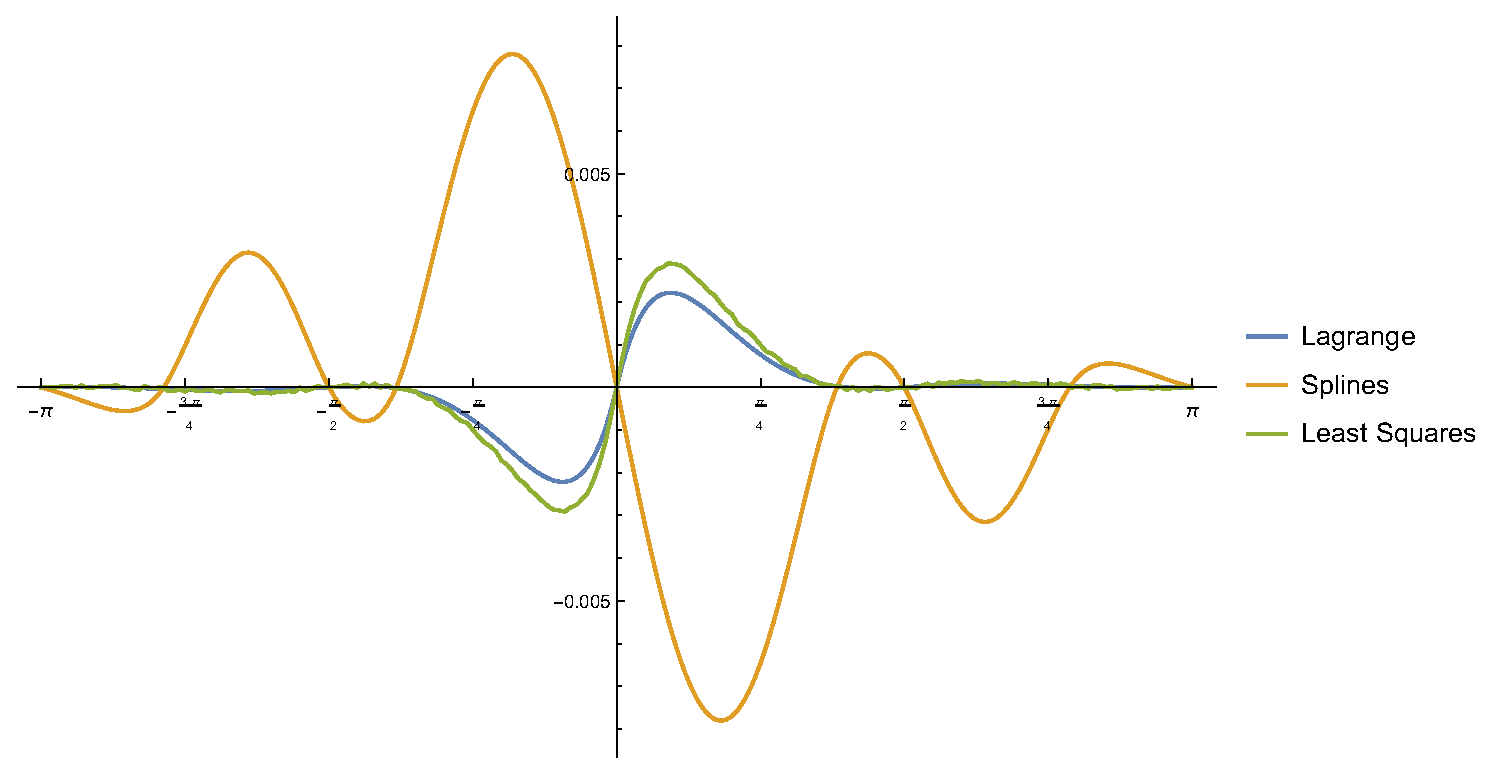
\includegraphics[width=\textwidth]{resources/graph.eps}
        \caption{Σφάλμα των μεθόδων}
        \label{fig:errorgraph}
\end{figure}

Για να εκτιμήσουμε τη σίγουρη ακρίβεια που μπορούμε να πετύχουμε θα βρούμε το μέγιστο σφάλμα για κάθε μέθοδο. Από τη συνάρτηση 
findMaxErr παίρνουμε:

\begin{table}[H]
    \centering
    \begin{tabular}{|l|l|}
    \hline
    Μέθοδος                                                                    & Μέγιστο Σφάλμα \\ \hline
    Lagrange                                                                   & 0.0022    \\ \hline
    Splines                                                                    & 0.0078      \\ \hline
    \begin{tabular}[c]{@{}l@{}}Ελάχιστα \\ τετράγωνα(βαθμού 8)\end{tabular}    & 0.0029  \\ \hline
    \end{tabular}
    \caption{Μέγιστα σφάλαματα}
    \label{tab:max-err}
\end{table}
Έτσι συμπεραίνουμε ότι με όλες τις μεθόδους πετυχαίνουμε ακρίβεια 2 δεκαδικών ψηφίων, αφού το μέγιστο σφάλαμα κάθε μεθόδου είναι 
μικρότερο του $10^{-2}$.

\subsection*{Άσκηση 6}
Οι συναρτήσεις της άσκησης περιέχονται στο φάκελο scripts/ex6.
\subsubsection*{Μέθοδος Τραπεζίου}
Έχω 11 σημεία στο $[0,\frac{\pi}{2}]$, άρα έχουμε $h=\frac{\frac{\pi}{2} - 0}{11-1}=\frac{\pi}{20}\simeq 0.1571$. Άρα τα σημεία είναι τα:
\begin{center}
    $\left\{0,\frac{\pi }{20},\frac{\pi }{10},\frac{3 \pi }{20},
    \frac{\pi }{5},\frac{\pi }{4},\frac{3 \pi }{10},\frac{7 \pi }{20},\frac{2 \pi }{5},\frac{9 \pi }{20},\frac{\pi }{2}\right\}$
\end{center}
Από τη συνάρτηση sinIntegralTrapezoidal παίρνουμε ότι $\int_0^{\frac{\pi}{2}}\sin(x)dx = 0.9979$. Το θεωρητικό σφάλμα προσέγγισης 
δίνεται από τον τύπο $\left| e \right| \leq \frac{(b-a)^3}{12N^2}M$ όπου $N$ ο αριθμός των διαμερίσεων και $M = max_{x\in[a,b]}\{ \left| f''(x) \right| \}$.
Στην περίπτωση που εξετάζουμε $N=10$ και $f(x) = \sin(x), f'(x) = cos(x), f''(x) = -sin(x)$ άρα $\left| f''(x) \right| = \sin(x)$. Επειδή $\sin(x)$ γνησίως 
αύξουσα στο $[0,\frac{\pi}{2}]$ έχει τη μέγιστη τιμή της στο $\frac{\pi}{2}$ και είναι ίση με $\sin(\frac{\pi}{2}) = 1$. Άρα:
\begin{equation*}
    \left| e \right| \leq \frac{(\frac{\pi}{2}-0)^3}{12 \cdot 10^2}\cdot 1 = \frac{\pi^3}{8\cdot 12\cdot 100} \simeq 0.0032
\end{equation*}
Υπολογίζουμε το ολοκλήρωμα $\int_0^{\frac{\pi}{2}}\sin(x)dx = \left[ -\cos(x) \right]_0^{\frac{\pi}{2}} = \cos(0) = 1$. Άρα το πραγματικό σφάλμα είναι: 
$1 - 0.9979 = 0.0021$.
\subsubsection*{Μέθοδος Simpson}
Εκτελούμε τώρα τη συνάρτηση sinIntegralSimpson η οποία δίνει ως αποτέλεσμα $\int_0^{\frac{\pi}{2}}\sin(x)dx = 1.0000033922209$. Το αριθμητικό σφάλμα είναι 
$1-1.0000033922209= -0.0000033922$. Το θεωρητικό σφάλμα δίνεται από τον τύπο: $\left| e \right| \leq \frac{(b-a)^5}{180N^4}M$ με $M=max_{x\in[a,b]}\{ \left| f^{(4)}(x) \right| \}$. 
Έχουμε ότι $f^{(4)}(x) = sin(x)$, άρα $M=1$. Εφαρμόζοντας στον τύπο:
\begin{equation*}
    \left| e \right| \leq \frac{(\frac{\pi}{2}-0)^5}{180\cdot 10^4}\cdot 1 = \frac{\pi^5}{32 \cdot 180 \cdot 10000} = 5.3128\cdot 10^{-6}
\end{equation*}

\subsection*{Άσκηση 6}
Τα γενέθλιά μου ήταν στις 18 Σεπτεμβρίου 2019. Οι 2 μετοχές που επέλεξα είναι: ΟΡΓ/ΣΜΟΣ ΠΡΟΓΝΩΣΤΙΚΩΝ ΑΓΩΝΩΝ ΠΟΔ/ΡΟΥ Α.Ε (ΟΠΑΠ) και 
ΑΕΡΟΠΟΡΙΑ ΑΙΓΑΙΟΥ Α.Ε.Ε. (ΑΡΑΙΓ). Οι συναρτήσεις OPAP και ARAIG παίρνουν 2 παραμέτρους: Τον αριθμό των συνεδριάσεων μετά την συνεδρίαση στις 
4/9/2019 και το βαθμό του πολυωνύμου με το οποίο θα προσεγγίσουμε τη συνάρτηση. Η συνάρτηση compare(n) επιστρέφει το μέσο σφάλμα για τις τιμές που 
έχουμε διαθέσιμες, όταν προσεγγίζουμε με πολυώνυμο βαθμού n. Εκτελώντας για n=2,3,4 παίρνουμε:

\begin{table}[H]
    \centering
    \begin{tabular}{|l|l|l|l|}
    \hline
    Βαθμός & 2      & 3      & 4      \\ \hline
    OPAP   & 0.0975 & 0.0554 & 0.0266 \\ \hline
    ARAIG  & 0.0703 & 0.0687 & 0.0449 \\ \hline
    \end{tabular}
    \caption{Μέσο σφάλμα προβλέψεων}
    \label{tab:stock-comparison}
\end{table}

Κάνουμε τώρα πρόβλεψη για την τιμή των μετοχών στις 18/09/2019, δηλαδή 10 συνεδριάσεις μετά τις 04/09/2019.

\begin{table}[H]
    \centering
    \begin{tabular}{|l|l|l|l|}
    \hline
    Βαθμός & 2      & 3      & 4      \\ \hline
    OPAP   & 9.8493 & 10.2792 & 9.8042 \\ \hline
    ARAIG  & 7.9895 & 7.8987 & 7.6142 \\ \hline
    \end{tabular}
    \caption{Πρόβλεψη για τις 18/9/2019}
    \label{tab:stock-prediction-1}
\end{table}

Η πραγματική τιμή της μετοχής ΑΡΑΙΓ στις 18/9 ήταν 8.1200 ενώ της ΟΠΑΠ 9.9000. 
Υπολογίζουμε και για 5 συνεδριάσεις μετά τις 18/9, δηλαδή στις 25/9.

\begin{table}[H]
    \centering
    \begin{tabular}{|l|l|l|l|}
    \hline
    Βαθμός & 2      & 3      & 4      \\ \hline
    OPAP   & 9.7215 & 14.7502 & 0.9885 \\ \hline
    ARAIG  & 8.3940 & 7.3314  & -0.9112 \\ \hline
    \end{tabular}
    \caption{Πρόβλεψη για τις 25/9/2019}
    \label{tab:stock-prediction-2}
\end{table}

Οι πραγματικές τιμές στις 25/9 για τις ΟΠΑΠ και ΑΡΑΙΓ ήταν 9.6050 και 8.0100, αντίστοιχα. Συγκρίνοντας τις προβλεπόμενες 
τιμές για τις 18/9 και τις 25/9 παρατηρούμε ότι και στις 2 ημερομηνίες και για τις 2 μετοχές το πολυώνυμο δευτέρου βαθμού 
είναι αυτό που κάνει προβλέψεις που είναι πιο κοντά στις πραγματικές τιμές των μετοχών. Ταυτόχρονα, τα πολυώνυμα τρίτου 
και τέταρτου βαθμού κάνουν προβλέψεις που διαφέρουν κατά πολύ από την πραγματική τιμή, με το πολυώνυμο του τέταρτου βαθμού να 
κάνει μέχρι και αρνητική πρόβλεψη στην τιμή. Από τα δεδομένα συμπεραίνουμε ότι τα πολυώνυμα μεγαλύτερου βαθμού, ενώ προσαρμόζονται 
καλύτερα στα δεδομένα που έχουμε, δεν είναι τόσο καλά στις προβλέψεις αφού είναι πιο ``απότομα'', δηλαδή αφού τελειώσουν όλα τα 
σημεία αυξάνεται πολύ απότομα η κλίση τους. Αντίθετα, η συνάρτηση 2ου βαθμού είναι πιο ομαλή, κάνει μεγαλύτερη καμπύλη, άρα 
κάνει και καλύτερες προβλέψεις. Παρακάτω φαίνονται οι γραφικές παραστάσεις των συναρτήσεων ελαχίστων τετραγώνων βαθμού 2,3,4 για 
τη μετοχή ΟΠΑΠ.

\begin{figure}[H]
    \centering
        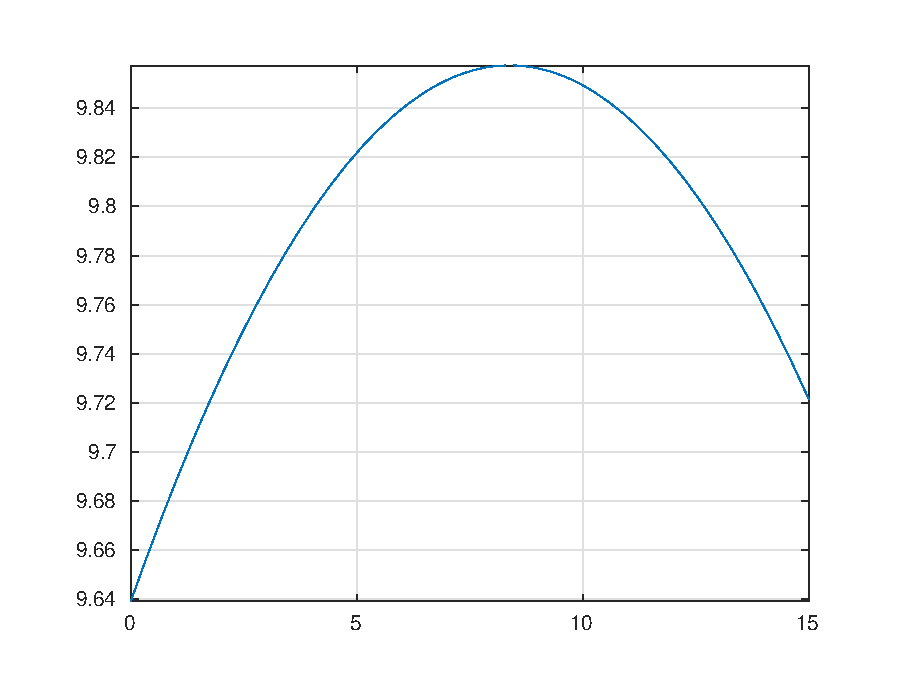
\includegraphics[width=.3\textwidth]{resources/opap2.eps}
        \includegraphics[width=.3\textwidth]{resources/opap3.eps}
        \includegraphics[width=.3\textwidth]{resources/opap4.eps}

        \caption{Γραφικές παραστάσεις ελαχίστων τετραγώνων}
        \label{fig:leastSquareComparison}
\end{figure}

\end{document}